\chapter{Diffusion and discussion of results}

This chapter aims to summarize the results of this thesis and to critically discuss them.
Moreover, the goal is to contextualize the results with existing literature to highlight their significance and facilitate comparisons.
This approach directly addresses the primary research question posed in this thesis: ``Can Boltzmann Machines be efficiently implemented on a physics-inspired hardware accelerator through analog noise injection?''
It also specifically responds to the secondary sub-question: ``How does the performance of the \ac{mem-HNN} accelerator compare to other hardware accelerators documented in the literature?''
While a detailed benchmark of conventional computing concepts is not part of this thesis, wherever possible a generalization of results should be established for an initial comparison.
Guided by this, more detailed comparisons can then be performed as part of future research

\section{Solution architecture and Hyperparameter tuning}

The first result is the developed Simulator Pipeline shown in fig.\ref{Overall architecture} as overall solution architecture. 
The required components for the combination of the digital computer with the \ac{mem-HNN} accelerator 
are universally valid and can be used to train Boltzmann Machines with the Hopfield Neural Network as sampling method. 
This is evaluated on the resulting \ac{IT}-artifact of the \ac{DSR} process by a test workload, where the \ac{mem-HNN}
achieves successful training with good prediction accuracies comparable to conventional training methods. 

The hardware-aware Simulation Pipeline implemented as part of the incremental \ac{IT}-artifact allows to predict the speed and energy consumption of the hardware long before any chips become available.
Such simulations are commonly used as part of the \ac{ASIC} design process and are known to produce relevant performance estimates.
Crucially, the simulator acts as a drop-in replacement, where the simulator correctly imitates the hardware's components and can be replaced by the actual hardware once it becomes available.

In the next step, the baselines for training are established using Gibbs sampling and the Metropolis-Hastings algorithm.
\textbf{Gibbs Sampling} is the most \textbf{sensitive} method and has a prediction accuracy of \(\mathbf{92.29\%}\), while
\textbf{Metropolis Hastings} is far more stable with a faster learning curve and a total prediction accuracy of \(\mathbf{94.15\%}\).
With the created Baselines, the implementation of the noisy injected Hopfield Network is achieved, which is considered the main result for the thesis. 
A complete training of the test workload is accomplished using a noisy \ac{mem-HNN}, where noise is introduced by injecting a random Gaussian distribution.
This process generates the stochastic activation function of the \ac{RBM}, as depicted in fig.\ref{Noisy_acitivation_function_good}.
Then, the performance of training is evaluated on the basis of the prediction accuracy of a machine learning pipeline consisting of an \ac{RBM} combined with a linear classifier.
Primarily, the metric ``prediction accuracy'' is of interest, since this helps to compare the performance with the other two conventional sampling methods.

Hence, the \textbf{asynchronously Hopfield Network} achieved a baseline of \(\mathbf{90.81\%}\) without Hyperparameter tuning but has a more stable  learning rate than Gibbs Sampling and
is equal to Metropolis-Hastings.
Here, the Hyperparameter tuning can be highlighted due to the fact that until now there was no data available for such an \ac{IT}-artifact and especially not for the Hopfield Network sampling method.
With some adjustments made to the standard deviation, which represents the standard deviation of the injected noise the stability, of the performance is measured.
The outcome is at a scale of 1.6 the prediction accuracy is the highest of all with a value of \(\mathbf{94.77\%}\) shown in \ref{Hyperparamers_Scale_ohne}.
In comparison, the \textbf{N/2 Half Hopfield Network} has a scale that is \textbf{more sensitive} than the asynchronous approach \ref{Hyperparamers_Scale_mit}.
On the other hand, its prediction accuracy of \(\mathbf{94.76\%}\) is very similar.
In contrast, noticeable differences can be seen when looking at the second Hyperparamer ``sampling iterations''. 
Here, the \textbf{asynchronously Hopfield Network} approach requires at least \textbf{4000 iterations} to achieve good results topping out with
a prediction accuracy of \(\mathbf{94.5\%}\) at 15000 sampling iterations. 
Meanwhile, the \textbf{N/2 Half Hopfield Network} updates, on average, 50\% of all neurons in the network per sampling iteration.
This results in achieving good prediction accuracy after just \textbf{221 sampling iterations}.
Hence, the best prediction accuracy with \(\mathbf{95.1\%}\) is the best out of all approaches with the least sampling iterations \ref{Hyperparamers_Iteraions_mit}.
Compared to the asynchronous update it is about \(\mathbf{18.09x}\) more efficient. 
Furthermore, compared to Metropolis-Hastings, which uses 10000 sampling iterations it is \(\mathbf{45.24x}\) more efficient.
Therefore, the N/2 Half approach is promising and the Hyperparameter findings from 4.5, especially for the sampling iterations, can be \textbf{generalized}.
Hence, the N/2 Half Hopfield Network updating approach for a Boltzmann Machine is at least equal in prediction accuracy but uses significantly fewer sampling iterations to the single spin update or Metropolis-Hastings.
In general, this shows Boltzmann Machines can be implemented on the physics-inspired hardware accelerator by analog noise injection. 

It is important to keep in mind that this is only comparable to the workload of the handwritten digit recognition by Scikit Learn that was tested on. 
It is to assume that the performance for other workloads and datasets would perform similar but need to be evaluated further. 
Hence, a literature comparison is difficult since parameters and data differ. 

\section{Throughput}

The second goal of this thesis's research question is to find out about the performance of the solution in terms of the 
computing speed (throughput) and energy efficiency. 
For the throughput the result of the \textbf{autocorrelation is important} to determine when a sampling method produces statistically independent configurations shown in fig.\ref{Autocorr comparison}.
The result of comparing Metropolis-Hastings, asynchronous Hopfield Network and N/2 Half Hopfield Network sampling the results are the following:
Metropolis Hastings can achieve independent samples after \textbf{100 sampling iterations}, while the asynchronous Hopfield approach requires around \textbf{200 sampling iterations} and therefore 
is \textbf{2x worse}. On the other hand, the \textbf{Hopfield Network} is \textbf{more stable} than Metropolis-Hastings and continuously needs around 200 iterations 
while Metropolis-Hastings needs around 400-500 iterations at the end of the training and is \textbf{more sensitive}. 
Next, the \textbf{N/2 Half Hopfield Network} approach only requires \textbf{3 sampling iterations} to be statistically independent of the previous sample.
Furthermore, it is \textbf{the most stable} out of all approaches. In comparison, N/2 Half updating is \(\mathbf{40x}\) faster than the single neuron
update and \(\mathbf{20x}\) faster than the Metropolis Hastings. 
Taking the average correlation time, the performance even increases to \(\mathbf{34x}\) faster than the single neuron Hopfield Network and \(\mathbf{46,6x}\)
faster than Metropolis-Hastings.
Lastly, it is worth mentioning that some outliers in the N/2 Half updating approach are found where 
the correlation does not fall below 1/e. This needs further research but effectively does not impact the training performance. 

When combining the autocorrelation with the technical specifications of the \ac{mem-HNN} accelerator following computing speed results arise:
The asynchronous Hopfield Network reaches a Throghput of \(\mathbf{10^6}\) samples per second with a high
consistency over the whole training period. 
Meanwhile, the N/2 Half Hopfield Network 
is around \(\mathbf{10^8}\) to \(\mathbf{10^9}\) samples per second with a more sensitive throughput and less consistency 
but overall higher throughput.
In numbers, the throughput of the N/2 Half Hopfield Network has an average of \textbf{144 megasamples/second} while the asynchronous update Hopfield Network has an average of \textbf{2,3 megasamples/second}.
The result shows that the N/2 Half approach is \(\mathbf{62,72x}\) faster. 

This can be put into comparison with literature values of \ac{FPGA}s since compared to a \ac{CPU} or \ac{GPU} it is the fastest accelerator.
One example of an \ac{FPGA} accelerator with 300MHZ used for Monte Carlo Simulations on Ising Models
performs one monte carlo step in \textbf{26.6ns} with a lattice size of 128 or \textbf{106.6ns} for a lattice size of 256.
A realistic estimate of 80ns for comparison is chosen. 
A Monte Carlo step in the paper is defined as once all spins have been touched.\footcite[cf.][4]{ortega-zamoranoFPGAHardwareAcceleration2016}
For the N/2 Half method, a script \texttt{touch\_all\_neurons.py} is used, which is part of the digital delivery, that calculates  
the average of iterations required to touch all neurons in the network.
With the calculated 8.79 iterations, the result is \(\mathbf{2ns * 8.79 = 17.58ns}\) per sampling step, which now is equivalent to one Monte Carlo step in the paper.
Therefore, the \ac{mem-HNN} is \(\mathbf{4.55x}\) faster for one sampling step than the \ac{FPGA} used.
Furthermore, the workload in this thesis is more complex than the 2D Ising Model in the paper and therefore an estimation for the same 
workload would be even more advantageous for the \ac{mem-HNN}. 
The frequency 300MHZ used by the \ac{FPGA} can be transformed to 3.33ns per clock cycle and with that a third graph can be added to figure\ref{Throughput comparison} showing the Metropolis-Hastings throughput.
This is achieved by using the 3.33ns and combining them with the results of \ref{Autocorr comparison}.
The resulting throughput comparison is shown in subsequent figure\ref{Comparison_throughput_literature_3}:
\begin{figure}[H]
    \centering
    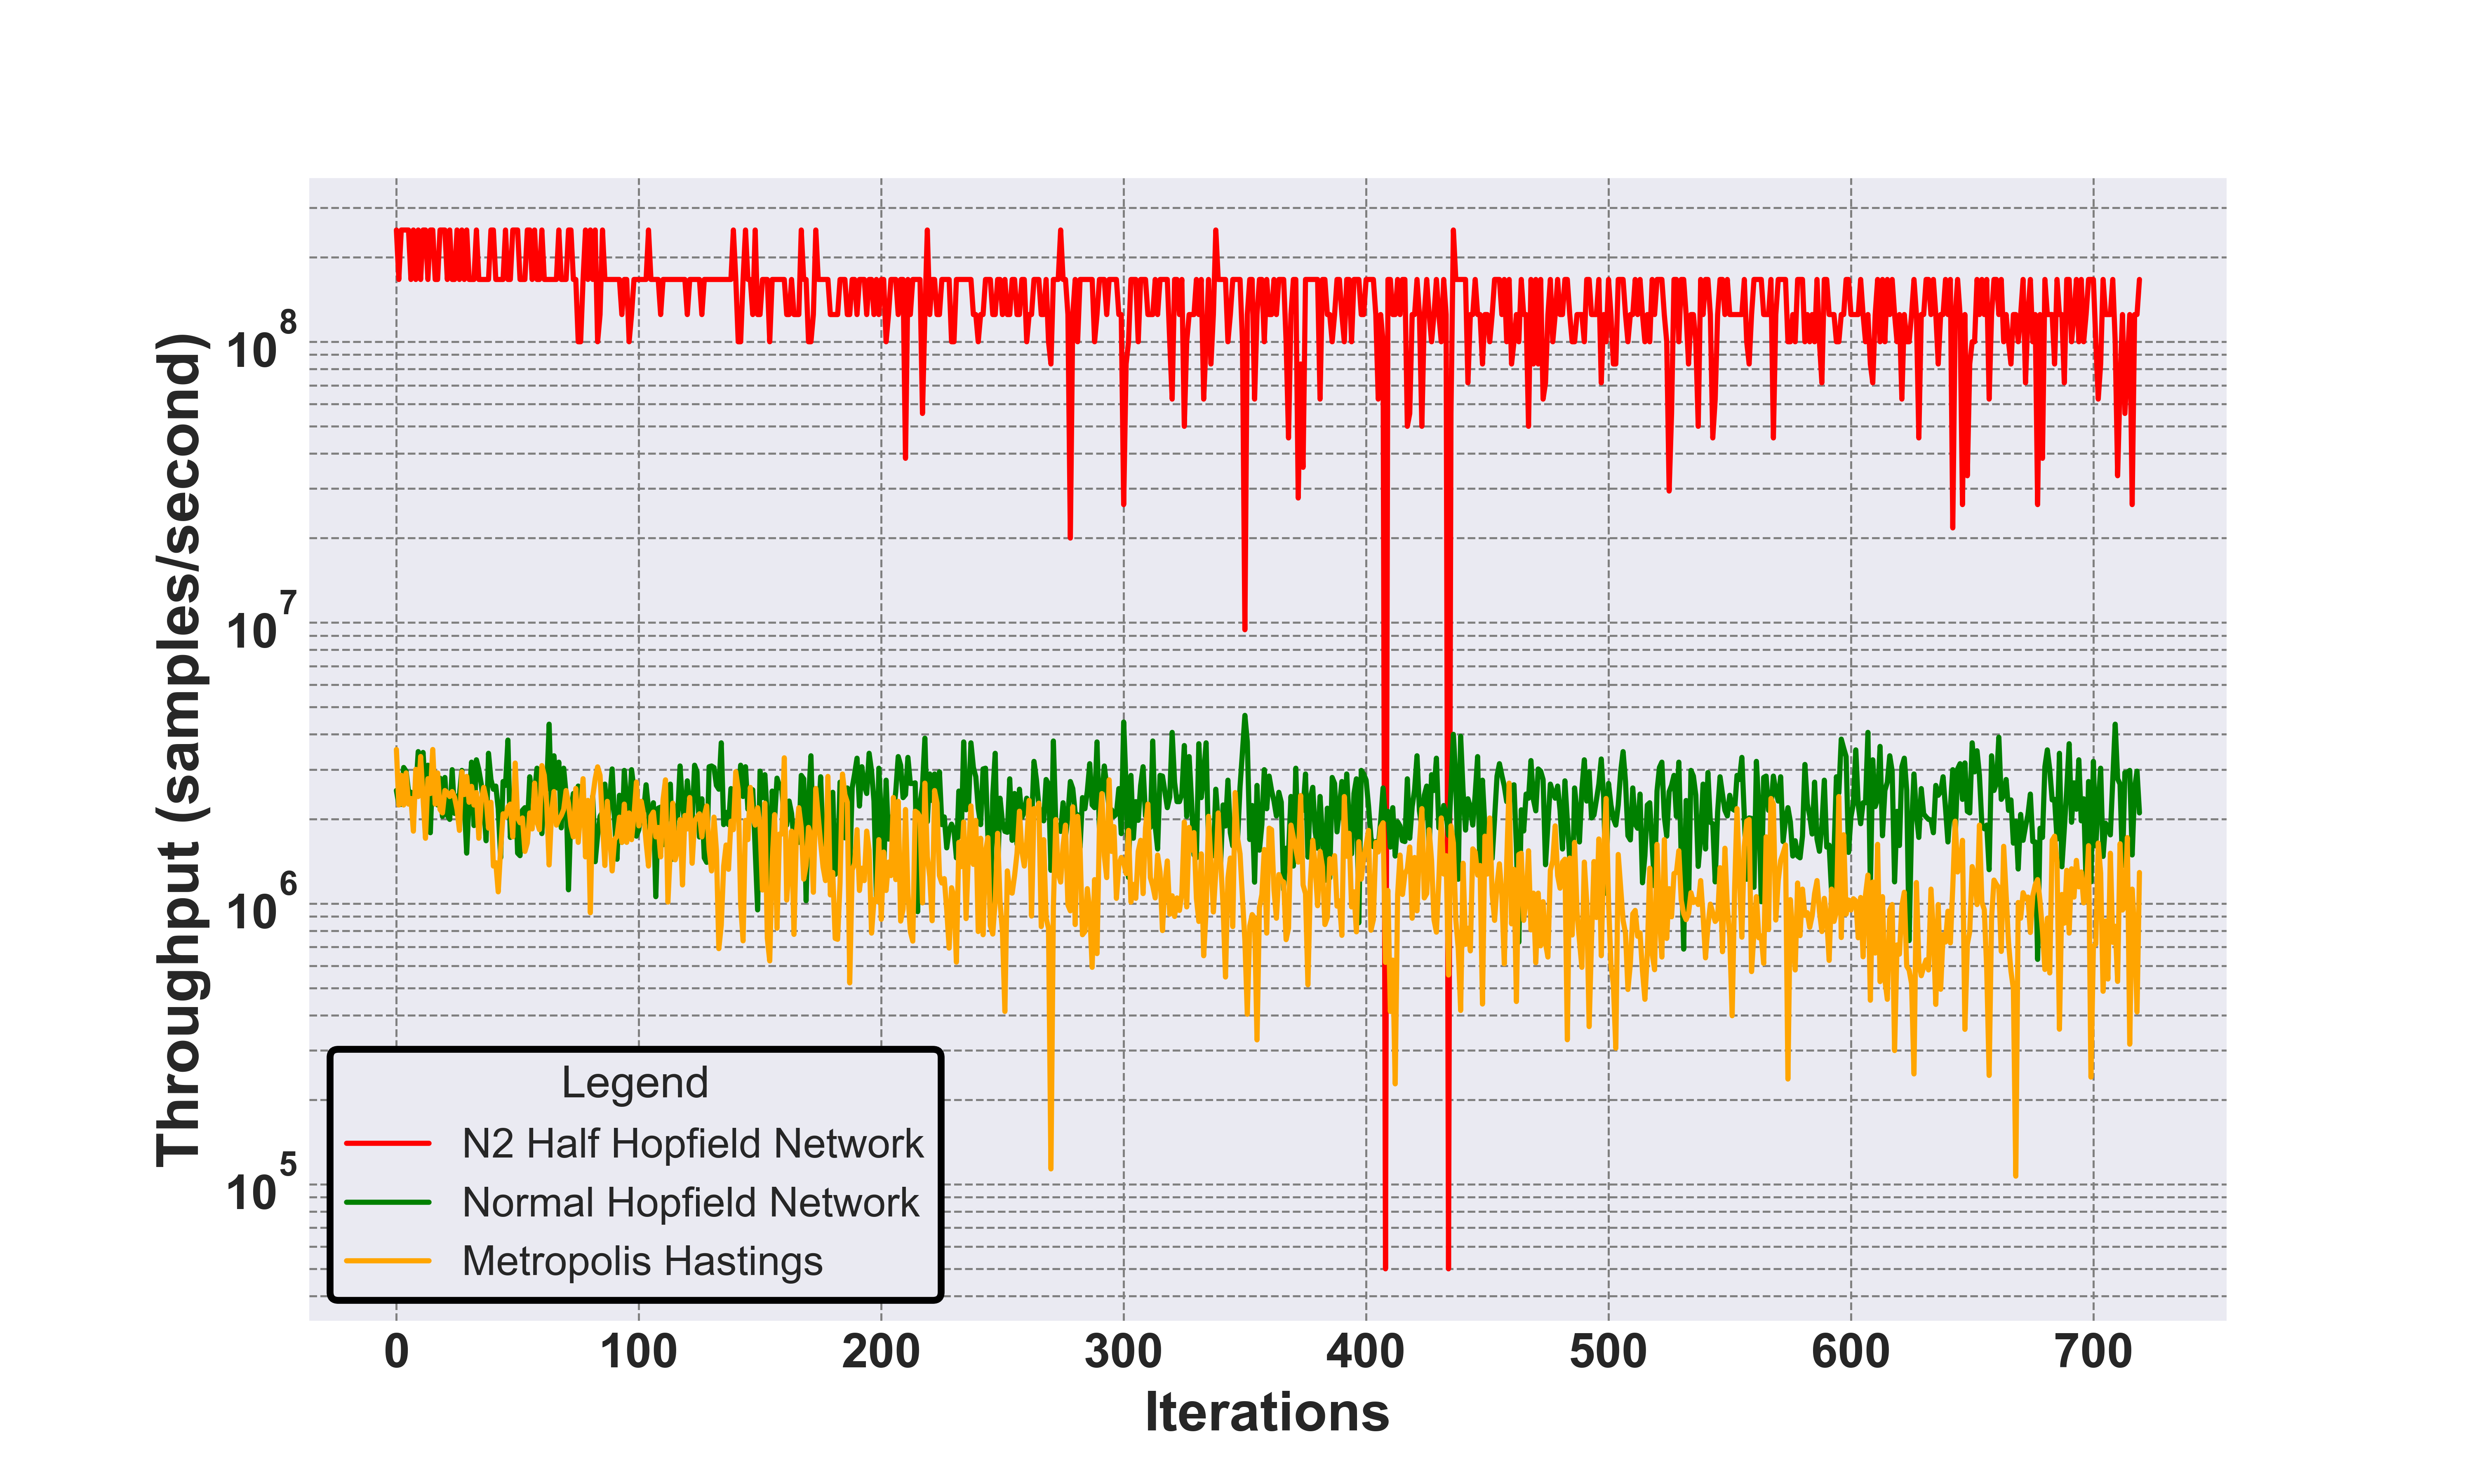
\includegraphics[width=0.8\linewidth]{graphics/Visualisierungen_throughput_MODIFIED.png}
    \caption{Comparison throughput literature}
    \label{Comparison_throughput_literature_3}
\end{figure}
The single-spin Hopfield Network initially matches the throughput of Metropolis-Hastings but eventually outperforms it.
The average throughput is \textbf{1.37 megasamples per second} for Metropolis-Hastings compared to \textbf{2.3 megasamples per second} for the Hopfield Network, making it \(\mathbf{1.67x}\) faster.
Lastly, another paper established a comparison of probabilistic hardware accelerators. Here, ``time per sweep(ns)'' is used, wich measures the duration required
once all spins have touched like in the other paper.\footcite[cf.][2]{aaditAcceleratingAdaptiveParallel2023}
A visual representation of the probabilistic accelerators can be seen in the following figure\ref{Comparison_throughput_literature_2}:
\begin{figure}[H]
    \centering
    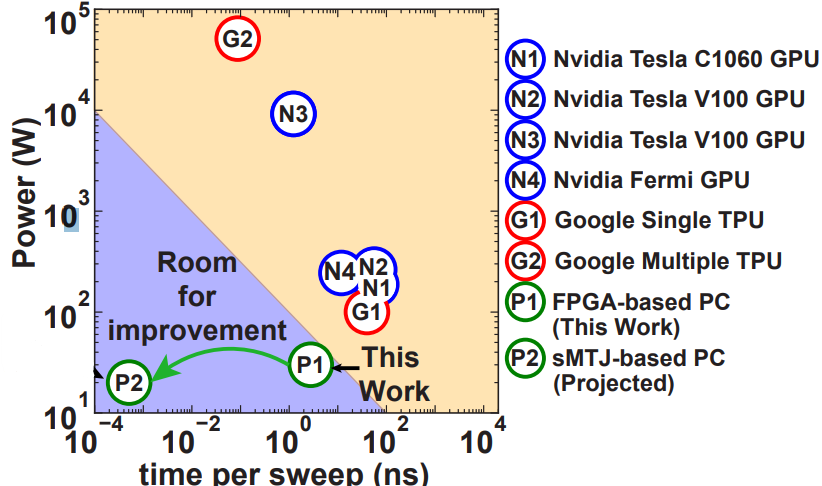
\includegraphics[width=0.50\linewidth]{graphics/Troughput_comparison.png}
    \caption{Comparison throughput with Metropolis Hastings}
    \label{Comparison_throughput_literature_2}
\end{figure}
With a clock cycle of 2 ns and the script used to ensure all 900 neurons in the network are updated, which requires 11.2 iterations, the resulting \ac{mem-HNN} time per sweep is \(\mathbf{22.4ns}\).
This is \textbf{slower} than the \ac{FPGA}-based PC (5.83ns) and Google’s multiple TPU (no exact value). 
It can be said that the research question is answered for throughput since the performance of the \ac{mem-HNN} is competitive. 
Although the time per sweep is competitive and surpasses some probabilistic accelerators it is important to consider that the workloads differ and a direct comparison is not possible requiring future work.
\section{Energy consumption}

Although the computation speed matches other probabilistic accelerators, this model's energy efficiency is distinctive.
Energy consumption per sampling iteration ranges from 50 to 20 picojoules, reducing as training progresses.
Power requirements start at \(\mathbf{22.5mW}\) and decrease to just below \(\mathbf{10mW}\), allowing the neural network to complete training with only 
\(\mathbf{6 mJ}\) across 720 iterations.
Although it is a simplistic comparison, one might consider, for instance, measuring the time it takes to run RBM training using the Metropolis-Hastings algorithm on a \ac{CPU}.
Training on a CPU\footnote{\texttt{Intel i7-10610U, 1.80GHz, 2304 Mhz, 4 Core(s), 8 Logical Processor(s)}} takes about 30 minutes with a thermal design power of 15W, consuming \textbf{27.000 Joules}
—\(\mathbf{460.000x}\) more energy than the \ac{mem-HNN}.
To make the comparison fairer, future work will include the energy consumption of the \ac{mem-HNN}'s communication, memory, and controller, which may slightly worsen the results.
The results in fig.\ref{Comparison_throughput_literature_2} display performance for a system with 7200 neurons.
To estimate energy for this neuron count, it is assumed that power consumption scales linearly with neuron number due to the implementation that subdivides into smaller subproblems, each equivalent to a single small-scale \ac{mem-HNN}.
Therefore, the power consumption of the \ac{mem-HNN} is calculated by multiplying by the factor 7200/164=43.\footcite[cf.][2]{aaditAcceleratingAdaptiveParallel2023}
The estimated power is \(\mathbf{\sim1W}\), making it \(\mathbf{10x}\) to \(\mathbf{1000x}\) more efficient than FPGA-, GPU-, and TPU-based sampling methods.
Overall, the \ac{mem-HNN} offers competitive computing speeds with a significant advantage in energy efficiency.
Therefore, Boltzmann Machines can indeed be efficiently implemented on the physics-inspired Hardware accelerator by analog noise injection answering the research question ultimately. 
Since the aim is to achieve new applications for more sustainable AI models on this \ac{ASIC} accelerator, 
this shows there can be large upside potential for running workloads on \ac{mem-HNN} chips.

\section{diffusion}
Now that the results have been processed and are comparable, the diffusion phase of the \ac{DSR} framework 
requires that results are made available to the public. 
The results and implementation are handed over to Hewlett Packard Labs and are used as 
bases for further research.
The goal is to further develop the model on the physical hardware accelerator and present the results in an upcoming paper at TechCon, HPE's internal research conference.
Additionally, the findings will be showcased at future scientific conferences and shared with HPE's research partners in the context of the \ac{mem-HNN}.
Lastly, this bachelor thesis is submitted to DHBW-Stuttgart for assessment. 
